\section{Структура базы данных}

\indent Из раздела \ref{sec:choose} очевидно, что в постоянной базе данных необходимо хранить информацию, на основе которой производится расчет объемно-календарного и оперативного планов.
Для этого необходимо хранить:

\begin{itemize}
	\item данные о заказах;
	\item данные о типах продукции;
	\item данные о продукции, которая относится к каждому заказу;
	\item данные о самой последовательности операций и самих операциях для каждого типа продукции;
	\item данные о каждой модели ресурсов;
	\item данные о связях между моделью ресурса и операциями.
\end{itemize}

\begin{figure}[ht]
	\centering
	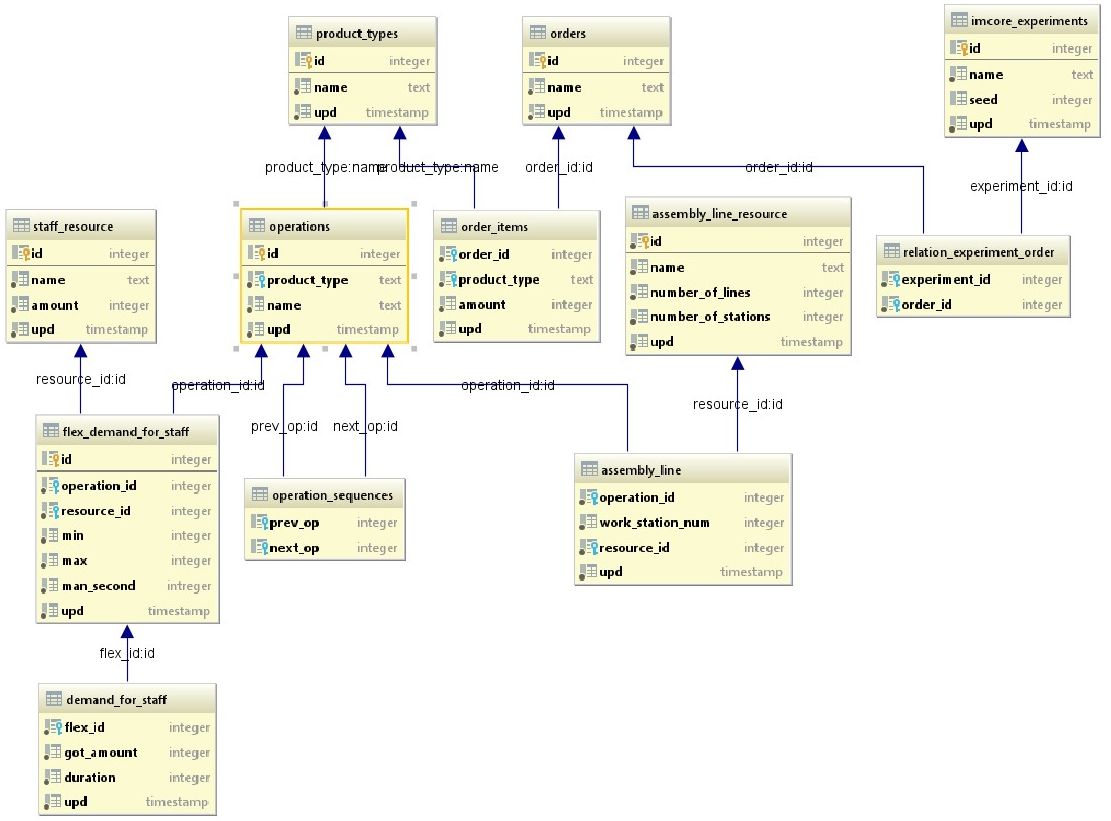
\includegraphics[width=\linewidth]{pics/databaseSchema.png}
	\caption{Схема базы данных}
	\label{fig:dbSchema}
\end{figure}

\indent Помимо этого, нужно учитывать, что кроме простого хранения данных, необходимо соблюдать ``версионность'', ввиду того, что карта технологического процесса может меняться во времени.
Значит и в базе данных требуется следить за тем, чтобы в любой момент времени было возможно использовать любую из версий данной карты, иначе новый расчет оперативного плана (при условии, что другие данные остались неизменными) приведет к созданию новой версии плана, а, следовательно, предыдущую версию восстановить будет либо очень сложно, либо, в худшем случае, невозможно.\\
\indent Для достижения данной цели в определенных таблицах было введено дополнительное поле - временная отметка обновления - ``upd''.
С помощью этой метки можно получить как последние данные из базы, просто максимизируя метку ``upd'', так и данные на определенный момент времени ограничивая эту метку необходимым временем.